%%%%%%%%%%%%%%%%%%%%%%%%%%%%%%%%%%%%%%%%%%%%%%%%%%%%%%%%%%%%%%%%%%%%%
%
% CSCI 1430 Writeup Template
%
% This is a LaTeX document. LaTeX is a markup language for producing
% documents. Your task is to fill out this
% document, then to compile this into a PDF document.
%
% TO COMPILE:
% > pdflatex thisfile.tex
%
% For references to appear correctly instead of as '??', you must run
% pdflatex twice.
%
% If you do not have LaTeX and need a LaTeX distribution:
% - Departmental machines have one installed.
% - Personal laptops (all common OS): www.latex-project.org/get/
%
% If you need help with LaTeX, please come to office hours.
% Or, there is plenty of help online:
% https://en.wikibooks.org/wiki/LaTeX
%
% Good luck!
% James and the 1430 staff
%
%%%%%%%%%%%%%%%%%%%%%%%%%%%%%%%%%%%%%%%%%%%%%%%%%%%%%%%%%%%%%%%%%%%%%
%
% How to include two graphics on the same line:
%
% \includegraphics[\width=0.49\linewidth]{yourgraphic1.png}
% \includegraphics[\width=0.49\linewidth]{yourgraphic2.png}
%
% How to include equations:
%
% \begin{equation}
% y = mx+c
% \end{equation}
%
%%%%%%%%%%%%%%%%%%%%%%%%%%%%%%%%%%%%%%%%%%%%%%%%%%%%%%%%%%%%%%%%%%%%%%%%%%%%%%%%%%%%%%%%%%%%%%%%

\documentclass[11pt]{article}

\usepackage[english]{babel}
\usepackage[utf8]{inputenc}
\usepackage[colorlinks = true,
            linkcolor = blue,
            urlcolor  = blue]{hyperref}
\usepackage[a4paper,margin=1.5in]{geometry}
\usepackage{stackengine,graphicx}
\usepackage{fancyhdr}
\setlength{\headheight}{15pt}
\usepackage{microtype}
\usepackage{times}
\usepackage{booktabs}

% python code format: https://github.com/olivierverdier/python-latex-highlighting
\usepackage{pythonhighlight}

\frenchspacing
\setlength{\parindent}{0cm} % Default is 15pt.
\setlength{\parskip}{0.3cm plus1mm minus1mm}

\pagestyle{fancy}
\fancyhf{}
\lhead{Project 1 Writeup}
\rhead{CSCI 1430}
\rfoot{\thepage}

\date{}

\title{\vspace{-1cm}Project 1 Writeup}


\begin{document}
\maketitle
\vspace{-2cm}
\thispagestyle{fancy}

\section*{Instructions}
\begin{itemize}
  \item Provide an overview about how your project functions. 
  \item Describe any interesting decisions you made to write your algorithm.
  \item Show and discuss the results of your algorithm.
  \item Feel free to include code snippets, images, and equations.
  \item List any extra credit implementation and result (optional).
  \item Use as many pages as you need, but err on the short side.
  \item \textbf{Please make this document anonymous.}
\end{itemize}

\section*{Project Overview}

This project aims to implement two functions \verb|myfilter()| and \verb|gen_hybrid_image()|. Different types of filters are applied to images to test \verb|myfilter()| function. As for \verb|gen_hybrid_image()|, besides testing with extra pairs of images, the effect of image assignment sequence to image1 and image2 is also investigated.

\section*{Implementation Detail}

Here is the implemetation for \verb|myfilter()|. At first, shapes of the kernel and image are obtained and an error message is raised if the filter has an even-dimension. In order to support both grayscale and RGB pictures, the grayscale picture is reshaped to a 3d array, so that we don't need to worry about the dimensions difference between grayscale and RGB picture. Then, the image is padded with reflect mode on the hight and width dimension using \verb|np.pad()|. The kernel is flipped using \verb|np.flit()| as we want to realize convolution operation. After all above manipulations, the output is obtained by taken dot product between \verb|flipped_kernel| and \verb|padded_image|. 

I have tried two ways to obtain the final output. (Both are included in code block below) The first implementation is an ordinary way: using two for loop over the height and width dimesion of image and use \verb|np.tensordot()| to obtain the convolution output. The second implementation is using \verb|np.lib.stride_tricks.as_strided()| and \verb|np.einsum()| to avoid using for loop, which can shorten the excutation time from 2.6s to 0.08s, about 30 times faster.

At last, if the input image is grayscale, the output is reshaped back to 2D to keep the result the same dimension as the input.

\begin{python}
(k, l) = kernel.shape
(m, n, c) = image.shape
if (k * l) % 2 == 0:
    raise Exception("Output with even filters are not defined!")

Grayscale = False
if len(image.shape) == 2:
    Grayscale = True
    image = np.reshape(image, (image.shape[0], image.shape[1], 1))

padded_image = np.pad(image, ((k // 2, k // 2), (l // 2, l // 2), (0, 0)), "reflect")
# because we want to calculate convolution, we need to flip the kernel
flipped_kernel = np.flip(kernel)

# First Implementation
output = np.zeros(image.shape)
for i in range(m):
    for j in range(n):
        output[i, j] = np.tensordot(flipped_kernel, padded_image[i : i + k, j : j + l], axes=[(0, 1), (0, 1)])

# Second Implementation
expanded_image = np.lib.stride_tricks.as_strided(
        padded_image,
        shape=(
            m,
            n,
            c,
            k,
            l,
        ),
        strides=(
            padded_image.strides[0],
            padded_image.strides[1],
            padded_image.strides[2],
            padded_image.strides[0],
            padded_image.strides[1],
        ),
        writeable=False,
    )

output = np.einsum("xyzij, ij->xyz", expanded_image, flipped_kernel)

if Grayscale:
    output = output.reshape(output, (m, n))
filtered_image = output
\end{python}

\newpage
\section*{Result}

\begin{enumerate}
    \item Different filters are tested as implemented in file \verb|proj1_part1.py|. The results for the \verb|dog.bmp| are shown in Fig. 1 and all of them meet the expectation for the corresponding filters.
    
    \begin{figure}[h]
        \centering
        \includegraphics[width=5cm]{../results/identity_image.jpg}
        \includegraphics[width=5cm]{../results/blur_image.jpg}
        \includegraphics[width=5cm]{../results/large_blur_image.jpg}
        \includegraphics[width=5cm]{../results/sobel_image.jpg}
        \includegraphics[width=5cm]{../results/laplacian_image.jpg}
        \includegraphics[width=5cm]{../results/high_pass_image.jpg}
        \caption{\emph{Left:} (from top to bottom)identity filter, large blur filter, laplacian fliter. \emph{Right:} (from top to bottom) blur fliter, sobel fliter, high pass fliter.}
    \end{figure}

    \item For the hybrid image generation, it will differ depending on which image is assign as image1 (which will provide the low frequencies) and which image
    is asign as image2 (which will provide the high frequencies). One simple example is presented below.
    \begin{figure}[h]
        \centering
        \includegraphics[width=10cm]{../results/hybrid_image_scales_1.jpg}
        \includegraphics[width=10cm]{../results/hybrid_image_scales_2.jpg}
        \caption{\emph{Top:} image1 is dog.bmp and image2 is cat.bmp \emph{Bottom:} image1 is cat.bmp and image2 is dog.bmp.}
    \end{figure}

\end{enumerate}

\newpage
\section*{Extra Credit (Optional)}
\begin{enumerate}
    \item Pad with reflected image content.
        \begin{python}
padded_image = np.pad(image, ((k // 2, k // 2), (l // 2, l // 2), (0, 0)), "reflect")
        \end{python}
    (Please check next page for 2 and 3)
    \newpage
    \item Create own hybrid image. Here is my own hybrid image result shown below.
    \begin{figure}[htbp]
        \centering
        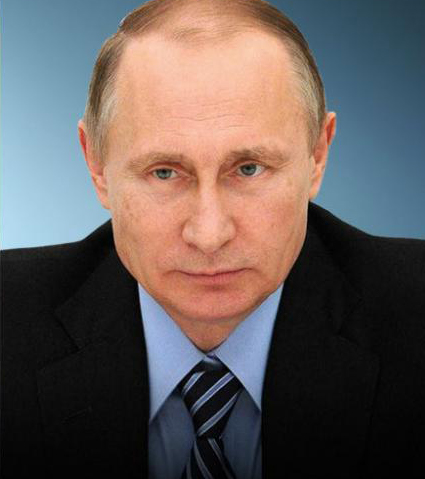
\includegraphics[width=5cm]{../data/Putin.jpg}
        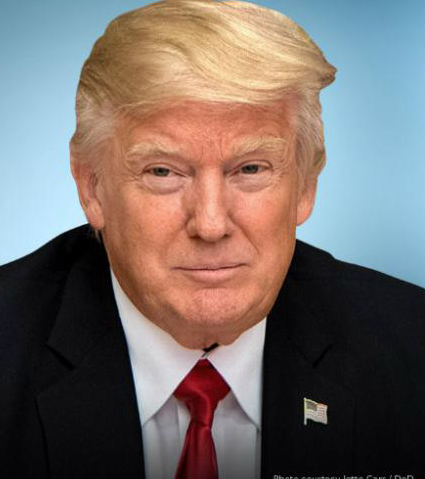
\includegraphics[width=5cm]{../data/Trump.jpg}
        \includegraphics[width=10cm]{../results/hybrid_image_scales.jpg}
        \caption{Own hybrid image: created from Putin.jpg and Trump.jpg}
    \end{figure}

    \item Here is the code for my FFT-based convolution. I use \verb|scipy.fftpack()| for the FFT transformation. It can produce similar images as presented in Fig. 1. However, I don't know why it hasn't passed the autograder.
        \begin{python}
(k, l) = kernel.shape
if (k * l) % 2 == 0:
    raise Exception("Output with even filters are not defined!")

Grayscale = False
if len(image.shape) == 2:
    Grayscale = True
    image = np.reshape(image, (image.shape[0], image.shape[1], 1))
(m, n, c) = image.shape
# because we want to calculate convolution, we need to flip the kernel
flipped_kernel = np.flip(kernel)
(k, l) = flipped_kernel.shape
padded_image = np.pad(
    image, ((k // 2, k // 2), (l // 2, l // 2), (0, 0)), "reflect",
)

fft_kernel = fftpack.fft2(flipped_kernel, shape=padded_image.shape[:2], axes=(0, 1))

fft_image = fftpack.fft2(padded_image, axes=(0, 1))
fft_output = fft_kernel[:, :, np.newaxis] * fft_image
output = fftpack.ifft2(fft_output, axes=(0, 1)).real
output = np.clip(output[k // 2 : -(k // 2), l // 2 : -(l // 2)], 0, 1)
if Grayscale:
    output = np.reshape(output, (m, n))
filtered_image = output
        \end{python} 
\end{enumerate}

\end{document}
